\section{Larger runtime costs for Compressed Sensing Reconstructions}\label{hypo}
The MeerKAT instrument produces a new magnitude of data volume. An image with several million pixels gets reconstructed from billions of Visibility measurements. Although MeerKAT measures a large set of Visibilities, the measurements are still incomplete. We do not have all the information available to reconstruct an image. Essentially, this introduces "fake" structures in the image, which a reconstruction algorithm has to remove. Additionally, the measurements are noisy.

We require an image reconstruction algorithm which removes the "fake" structures from the image, and removes the noise from the measurements. 



The inteferometer introduces two forms of corruption into the measurements:

The measurements are subjected to both noise and corruption from the instrument itself.  

 An image reconstruction algorithm should remove the 

Noisy measurements, and the instrument itself introduces "fake" image structures. Large scale image reconstruction problem. Several different reconstruction algorithms were developed for this problem, which can be separated into two classes: Algorithms based on CLEAN, which are cheaper to compute and Compressed Sensing based algorithms, which create higher quality reconstructions.

CLEAN uses a deconvolution

Compressed Sensing based algorithms have an image regularization. 
 
This project searches for a way to reduce the runtime costs of Compressed Sensing based algorithms.
 One of the reasons is that both algorithms use the non-uniform FFT Approximation, but Compressed Sensing algorithms need more non-uniform FFT Approximation than CLEAN.

We need the non-uniform FFT to transform. In the state-of-the-art Architectures, we need several non-uniform FFT operations for a single reconstruction. It is an expensive operation, 

we try to reduce the number of non-uniform FFT. One part of speeding up compressed Sensing reconstructions is reducing the number of non-uniform FFT approximations.

State-of-the-art CLEAN and Compressed Sensing algorithms use a similar Architecture, but with important differences.


\subsection{The Major Cycle Architecture}

\begin{figure}[h]
	\centering
	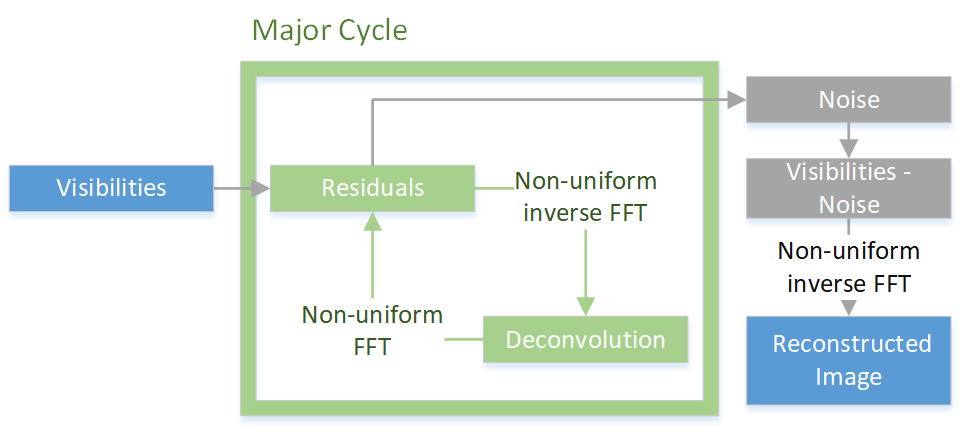
\includegraphics[width=0.80\linewidth]{./chapters/02.hypo/Major-Minor.png}
	\caption{The Major Cycle Architecture}
	\label{hypo:major}
\end{figure}


Figure \ref{hypo:major} depicts the Major Cycle Architecture used by CLEAN algorithms. First, the Visibilities get transformed into an image with the non-uniform FFT. The resulting image contains corruptions of the measurement instrument. A deconvolution algorithm, typically CLEAN, removes the corruption of the instrument with a deconvolution. The residual image, which should contain mostly noise, gets transformed back into residual Visibilities and the cycle starts over.

In the Major Cycle Architecture, we need several deconvolution attempts before it has distinguished the noise from the measurements. For MeerKAT reconstruction with CLEAN, we need approximately 4-6 non-uniform FFT cycles. 

CLEAN deconvolutions are not trivial to distribute.


\subsection{Compressed Sensing Architecture}\label{hypo:CSArch}

\begin{figure}[h]
	\centering
	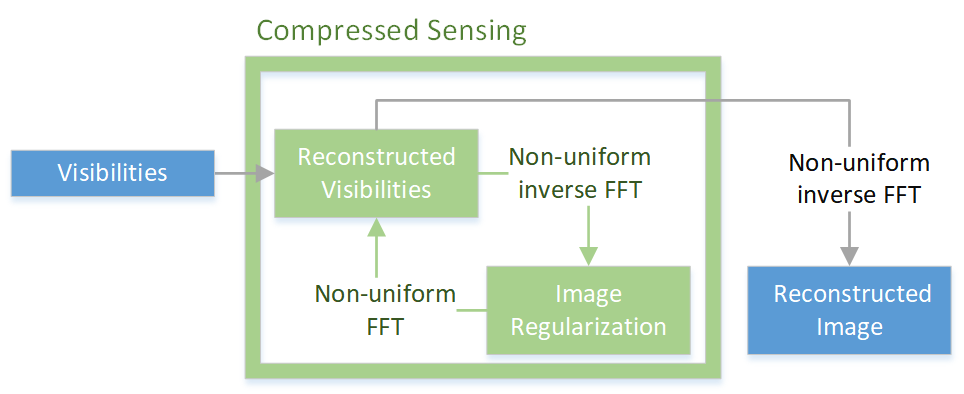
\includegraphics[width=0.80\linewidth]{./chapters/02.hypo/CS.png}
	\caption{State-of-the-art Compressed Sensing Reconstruction Architecture}
	\label{hypo:cs}
\end{figure}

Figure \ref{hypo:cs} depicts the architecture used by Compressed Sensing reconstructions. The Visibilities get transformed into an image with the non-uniform FFT approximation. The algorithm then modifies the image so it reduces the regularization penalty. The modified image gets transformed back to Visibilities and the algorithm then minimizes the difference between measured and reconstructed Visibilities. This is repeated until the algorithm converges to an optimum.

In this architecture, state-of-the-art Compressed Sensing algorithms need approximately 10 or more non-uniform FFT cycles to converge. It is one source for the higher runtime costs. There is one upside in this architecture: State-of-the-art algorithms managed to distribute the "Image Regularization" operation.

\subsection{Hypothesis for speeding up Compressed Sensing Algorithms}
Compressed Sensing Algorithms are not bound to the Architecture presented in section \ref{hypo:CSArch}. For example, we can design a Compressed Sensing based deconvolution algorithm and use the Major Cycle Architecture instead.

Our hypothesis is: We can create a Compressed Sensing based deconvolution algorithm which is both distributable and creates higher quality reconstructions than CLEAN. Because it also uses the Major Cycle architecture, we reckon that the Compressed Sensing deconvolution requires a comparable number of non-uniform FFT cycles to CLEAN. This would result in a Compressed Sensing based reconstruction algorithm with similar runtime costs to CLEAN, but higher reconstruction quality and higher potential for distributed computing.


